\section{Grundlegendes zu \textit{ROS} und Lubuntu}
\label{sec:grundlegendesROS-OS}   
Im Folgenden wird eine kurze Einleitung zu ROS\footnote[1]{http://www.ros.org/}  und dem Betriebssystem, das auf dem Auto installiert war, Lubuntu, gegeben. Diese Grundausstattung an Software war bei allen Gruppen identisch.
%%%%%%
\subsection{Was ist \textit{ROS}?}
Im Projektseminar wird die Middleware \textit{ROS} eingesetzt. \textit{ROS} steht für \textit{Robot Operating System} und wird heute vor allem von der \textit{Open Source Robotics Foundation} fortentwickelt. Die Software ist dabei kein klassisches Betriebssystem, wie der Name vermuten lässt, sondern eine Middleware, die auf einem der klassischen Betriebssysteme (aktuell werden Mac-OS und Linux stabil unterstützt) aufgespielt wird. \textit{ROS} sorgt für eine starke Hardware-Abstraktion, sodass fast beliebige Hardware eingesetzt werden kann und diese auch fast beliebig austauschbar ist. \textit{ROS} abstrahiert diese und stellt allgemeine Programmierschnittstellen bereit. Zudem ermöglicht \textit{ROS} eine einfache, standardisierte Kommunikation zwischen den Hard- und Softwarekomponenten.
Die drei wesentlichen Faktoren \textit{ROS} einzusetzen sind Modularität, Portabilität und Wiederverwendbarkeit, sowie eine vereinfachte Softwareentwicklung (einfache Interfaces, Debugging, Monitoring, Testen).

\begin{figure}[htbp] 
	\centering
	
\includegraphics[width=150pt]{images/rosorg-logo1.png}
	\caption{Logo von \textit{ROS}}
	\label{fig:LogoROS}
\end{figure}

%%%%%%
\subsubsection{Wie ist \textit{ROS} aufgebaut?}
\textit{ROS} besteht hauptsächlich aus drei Komponenten, die beliebig kombiniert und vernetzt werden können: \textit{Nodes}, \textit{Topics} und \textit{Services}. \textit{Nodes} sind Softwareknoten, die dafür zuständig sind, bereitgestellte Daten aufzunehmen und zu prozessieren. In den \textit{Nodes} ist die Intelligenz des Autos implementiert und dort werden durch die Sensorik gewonnene Daten in Befehle für die Aktorik des Autos umgesetzt. 
\textit{Topics} sind asynchrone Kommunikationslösungen, mit denen die Knoten Daten und Nachrichten, sog. \textit{Messages}, austauschen können. Dabei sind Produktion und Konsumption der Daten getrennt, indem \textit{Messages} an einer Stelle \textit{gepublished} werden, und anschließend dem gesamten System zum Abruf zur Verfügung stehen. Andere Knoten können diese Nachrichten nun Empfangen (\textit{subscribe}). Es ist also völlig unerheblich, wo genau die Daten herkommen, was bedeutet, das beliebig viele \textit{Nodes} die \textit{Topics publishen} können und beliebig viele sie wiederum \textit{subscriben} können. 
\textit{Services} sind synchrone Kommunikationsmöglichkeiten. Während \textit{Topics} einen n:m-Nachrichtenaustausch ermöglichen, sind Services dazu da, einen direkten 1:1-Nachrichtenaustausch zwischen zwei \textit{Nodes} zu ermöglichen. Ein \textit{Service} besteht dabei aus einem Nachrichtenpaar von Anfrage und Antwort auf diese. 

%%%%%%
\subsection{Betriebssystem}
Zu dem vorgegebenen Software Framework des Projektseminars gehörte neben \textit{ROS} ebenfalls das Betriebssystem \textit{Lubuntu} (auch mit Echtzeitkernel). \textit{Lubuntu} ist ein Derivat des Linux-Betriebssystems \textit{Ubuntu}, das \textit{LXDE} als Desktop-Umgebung verwendet. Linux ist allgemein bekannt, weshalb wir an dieser Stelle nicht mehr weiter darauf eingehen möchten. 
Zu bemerken ist jedoch, dass bei uns der Echtzeitkernel nicht zum Einsatz kam, da die Hardware des Autos durch unsere Implementierung nur zu ca. 30\% ausgelastet war. 

%%%%%%
\subsection{Welche Möglichkeiten von \textit{ROS} haben wir genutzt?}
Aufgrund unserer Codestruktur eines Zustandsautomaten, den wir in einem \textit{ROS-Node} implementiert haben, kamen wir mit wenigen \textit{ROS-Nodes} aus. Wie später beschrieben, haben wir lediglich drei \textit{Nodes} für das generelle Management der Sensorik und Aktorik, der Kamera und für die FSM (Finite State Machine/Zustandsautomat) benötigt. Wie gerade beschrieben, nutzen wir für die Kommunikation zwischen den einzelnen Codebausteinen ausschließlich \textit{Topics}.
Zur Kamerakalibrierung haben wir eine Kombination der von \textit{ROS} bereitgestellten Kalibrierungsmöglichkeiten und Methoden der \textit{OpenCV}-Bibliothek genutzt. Später in der Ausarbeitung werden wir noch ausführlicher auf die Details der Implementierung und Umsetzung eingehen.

\begin{figure}[htbp] 
	\centering
	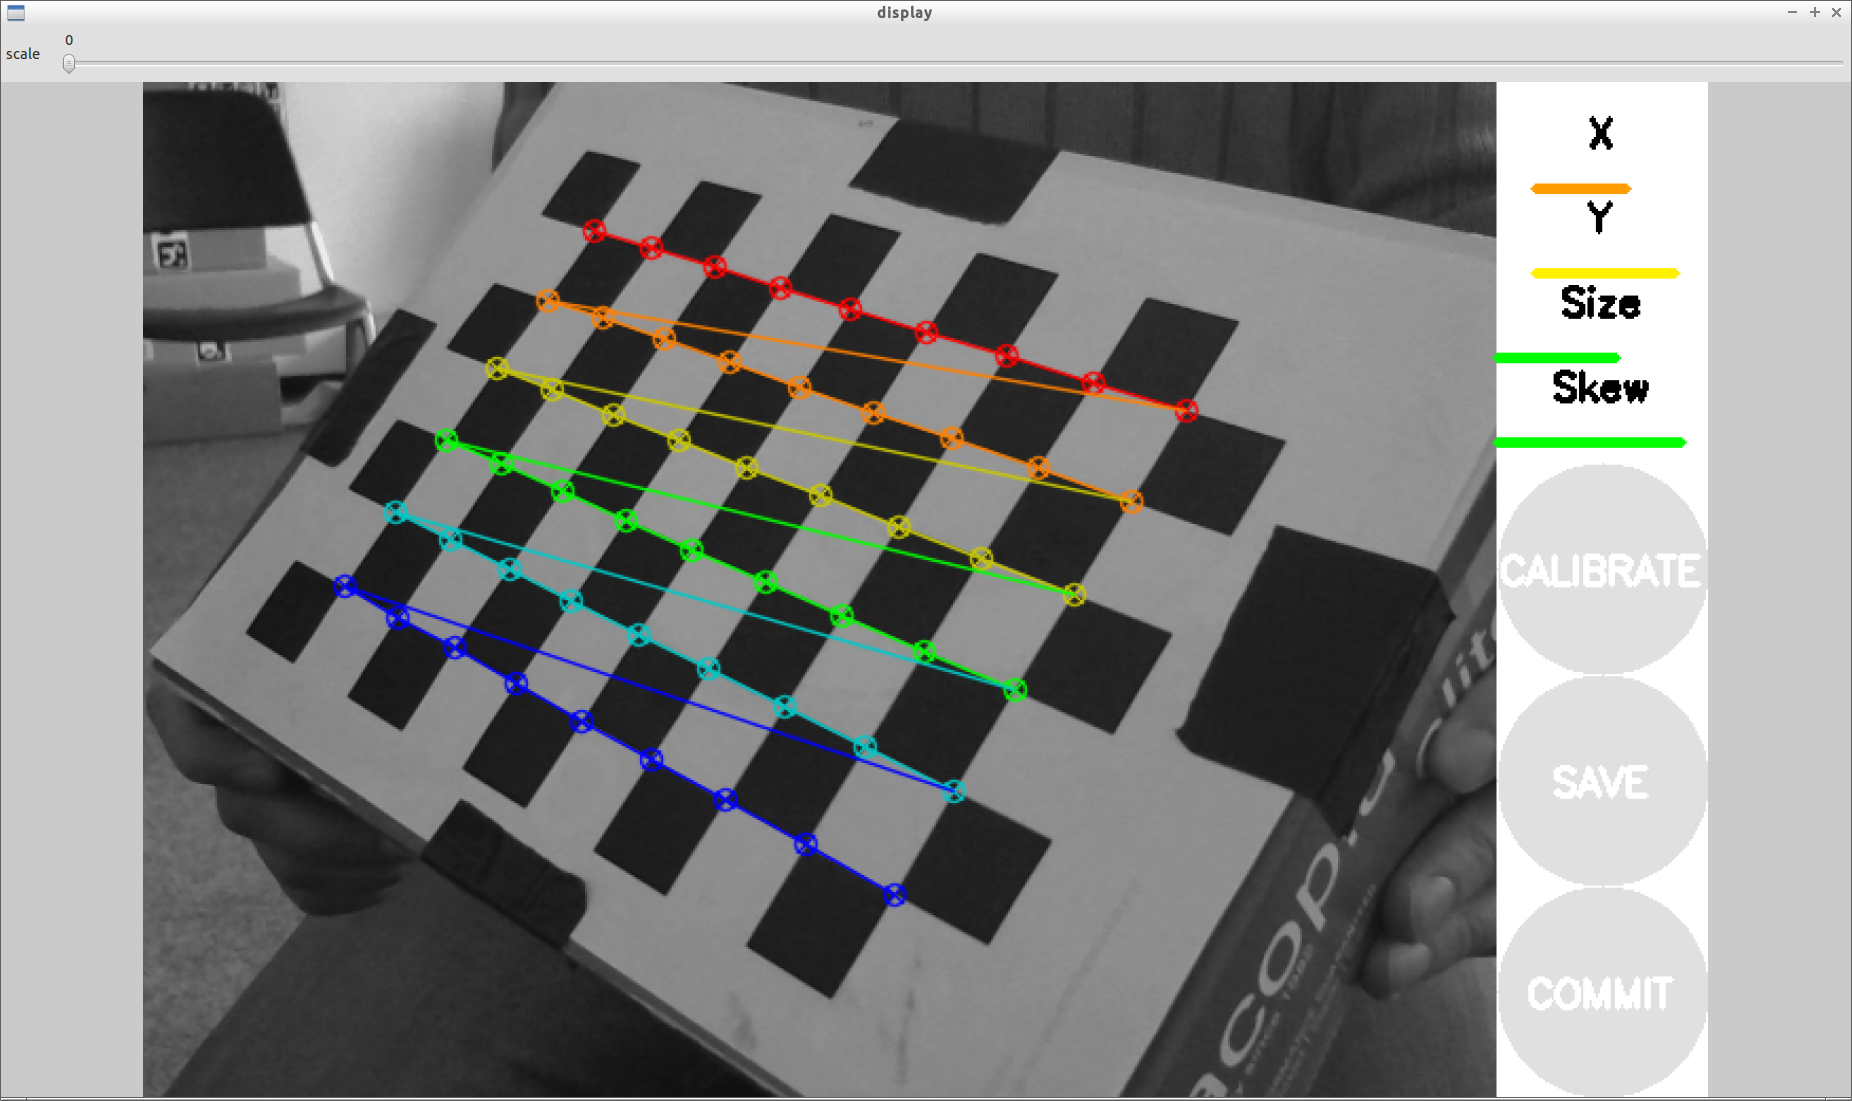
\includegraphics[width=\textwidth]{images/schachbrett.png}
	\caption{Kamerakalibrierung mit \textit{ROS}}
	\label{fig:CamKalib}
\end{figure}